\cleardoublepage
\chapter{Parametric study of HIFI's standing waves}
\chaptermark{Parametric study}

In this part, I use HIFI as an example.
My goal is to show where each standing wave in HIFI is born.
Introduce terms:
FPU
DSB
SSB
USB
LSB
IF

%=============================================================================

\section{Model used to explore the parameters}

\begin{figure}[hbtp]
    \centering
    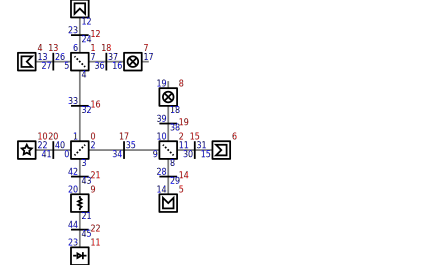
\includegraphics{ports_diplexerband}
    \caption{Networks and ports used in the model of a HIFI diplexer band.}
    \label{fig:ports_diplexerband}
\end{figure}

\begin{table}[hbtp]
    \begin{tabular}{rlll}
        \toprule
        nb & type & description & parameters \\
        \midrule
         0 & grid             & entry grid                      & \\
         1 & grid             & H diplexer grid                 & \\
         2 & grid             & V diplexer grid                 & \\
         3 & rooftop mirror   & mobile                          & \\
         4 & rooftop mirror   & immobile                        & \\
         5 & rooftop mirror   & mobile                          & \\
         6 & rooftop mirror   & immobile                        & \\
         7 & mixer            & H                               & \\
         8 & mixer            & V                               & \\
         9 & attenuator       &                                 & \\
        10 & source           & CBB, HBB or sky  & \\
        11 & local oscillator & source of noise                 & \\
        12 & distance         & variable       & \SI{22.5}{\milli\meter} + rooftop offset  \\
        13 & distance         &                                 & \SI{22.5}{\milli\meter}           \\
        14 & distance         & variable       & \SI{22.5}{\milli\meter} + rooftop offset  \\
        15 & distance         &                                 & \SI{22.5}{\milli\meter}           \\
        16 & distance         &                                 & \SI{40.0}{\milli\meter}           \\
        17 & distance         &                                 & \SI{40.0}{\milli\meter}           \\
        18 & distance         &                                 & \SI{196.5}{\milli\meter}          \\
        19 & distance         &                                 & \SI{196.5}{\milli\meter}          \\
        20 & distance         & to CBB, HBB or sky              & 1248.5 or 1343.5 or \SI{0}{\milli\meter} \\
        21 & distance         &                                 & \SI{745.85}{\milli\meter} \\
        22 & distance         &                                 & \SI{573.61}{\milli\meter} \\
        \bottomrule
    \end{tabular}
\end{table}

%=============================================================================
\section{Exploration}

At first, the whole system will be as perfect as I can make it.  I do not have a model for a perfect grid, but I can make the grid so thin and dense that it will drown the effect of the grid within the thickness of the line in the plots.

Then, little by little I will make the elements more realistic, and describe the results.

Each time, I present a plot of
\begin{itemize}
    \item the coupling of the mixers to the source before mixing,
    \item the coupling of the mixers to the LO before mixing,
    \item the sideband ration of the source.
    \item the sideband ratio of the LO.
    \item the coupling of the mixers to the source after mixing,
    \item the coupling of the mixers to the LO after mixing,
\end{itemize}

The source can be the sky or one of the calibration black bodies.

Why do the LO coupling matters?
Because the LO is a source of noise.
And a strong one, think \SI{120}{\kelvin}.
Of course, diplexer bands and beam splitter bands try to minimize the LO coupling, but even \SI{1}{\percent} of \si{120}{\kelvin} matters, remember that the CMB is at \SI{3}{\kelvin}.

Note that the 120 K noise is emitted in both polarizations.  That means 60 in H and 60 in V.

Define the sideband ratio.
Why does the SBR matter?  Why do we plot it?

Explain how I fold, and what it means.
It shows how the patterns in the upper and lower sideband interfere together.  Sometimes they construct,
sometimes they destrucs.
It is not a calibrated spectrum, but it shows the type of features that we expect to see on the continuum of a spectrum.


%-----------------------------------------------------------------------------
\clearpage
\subsection{Ideal instrument}

\begin{figure}[hbtp]
    \centering
    \begin{subfigure}[b]{.5\textwidth}
        \includegraphics{chapter_3/0_ideal_h_dsb}%
        \caption{H mixer power coupling.}
    \end{subfigure}%
    \begin{subfigure}[b]{.5\textwidth}
        \includegraphics{chapter_3/0_ideal_v_dsb}%
        \caption{V mixer power coupling.}
    \end{subfigure}%
    \\
    \begin{subfigure}[b]{.5\textwidth}
        \includegraphics{chapter_3/0_ideal_h_sbr}%
        \caption{H mixer sideband ratio.}
    \end{subfigure}%
    \begin{subfigure}[b]{.5\textwidth}
        \includegraphics{chapter_3/0_ideal_v_sbr}%
        \caption{V mixer sideband ratio.}
    \end{subfigure}%
    \\
    \begin{subfigure}[b]{.5\textwidth}
        \includegraphics{chapter_3/0_ideal_h_ssb}%
        \caption{H mixer folded coupling.}
    \end{subfigure}%
    \begin{subfigure}[b]{.5\textwidth}
        \includegraphics{chapter_3/0_ideal_v_ssb}%
        \caption{V mixer folded coupling.}
    \end{subfigure}%
    \caption{Coupling and sideband ratios of the H and V mixers for an ideal instrument.}
    \label{fig:0_ideal}
\end{figure}

A perfect instrument would couple \SI{100}{\percent} of the source and \SI{0}{\percent} of other noise sources at all frequencies.
Unfortunately, an instrument using diplexers for its LO injection is perfect for one frequency only.

\subsubsection{Purpose and functioning of the diplexers}
Here are a few words on the purpose and the functionning of the diplexer; for more details, refer to \cref{sec:annex_a}.

The mixers in HIFI require two inputs: a narrow-band high-power local oscilator signal, and the signal from the astronomical or calibration source.
Some mixers accept that these two signals come from different directions, but the mixers used in HIFI expect these two signals to arrive at normal incidence on the same surface.
Since placing the local oscilator in front of the source would occult the source, we need to find another way of injecting the LO signal into the source signal.
Solving this problem is the role of the entry grid (network 0 on \cref{fig:ports_diplexerband}): \SI{50}{\percent} of the source and \SI{50}{\percent} of the LO are sent to each mixer.

Now that each mixer receives polarized signal from the source, it makes sense for the mixers to reject the other polarization which is guaranteed to contain only noise:
this doubles the signal-to-noise ratio.
Unfortunately, the LO signal and the source signal have prependicular polarizations since they are combined with a wire grid polarizer.
If we want both to couple to the mixer, one of these two signals must be rotated by \SI{90}{\degree}.
Rotating one polarization is the role of the diplexer unit.
The diplexer rotates a polarization by splitting it in two and recombining it with a phase delay.

On \cref{fig:ports_diplexerband}, the H diplexer is made of the optical elements numbered 1, 3, 4, 12 and 14.
The V diplexer is made of 2, 5, 6, 14 and 15.
In each case: one grid, two rooftop mirrors, and two distances separating the rooftops from the grid.

For example, a vertical signal is separated by the diplexer grid into two components, one at \SI{-45}{\degree} and one at +\SI{+45}{\degree}. % Had troubles using 'retain-explicit-plus'.
Then, one of these two components is delayed by \SI{180}{\degree} relatively to the other one.
When recombined later by the grid, the result is a horizontally-polarized signal.

The phase delay used for rotating the polarization of the LO or the source signal is controlled by the distances between the diplexer grid and the rooftop mirrors.
The phase delay depends on the position of the rooftop mirror and the wavelength.
The position of the rooftop mirror is chosen such that the pathlengh difference makes one signal recombined in phase (not rotated) and the other signal in antiphase (rotated).
This is how we can give the same polarization to the LO signal at the LO frequency and the source signal at the LSB and USB frequencies frequencies.
The optimal coupling is achieved only for one specific frequency in each sideband.
For convenience, we place the peak of efficiency in the middle of the these sidebands as shown on \cref{fig:0_ideal}.
For all the other frequencies in these sidebands, the recombined signal is elliptically polarized, resulting in less source signal being coupled, and more LO noise being coupled.

\subsubsection{Model}

To model this ideal instrument, we 

The behavior of the diplexer explains the shape of the curves presented in \cref{fig:0_ideal}.
This coupling is the coupling that we expect from an ideal detector using a diplexer for its LO injection.
The coupling to the source is maximal at the center of the sidebands.
The coupling to the LO is minimal at the center of the sidebands but maximal at the LO frequency (not represented, but the LO curves reach 1 at the LO frequency of \SI{992}{\giga\hertz}).

The left column of \cref{fig:0_ideal} presents the power coupling of the H mixer.
The right column corresponds to the V mixer.
The H mixer is sensitive to the H polarization of the source and to the V polarization of the local oscillator: the local oscillator polarization started as V but was rotated by the diplexer to line up with H when hitting the mixer.
Since the entry grid is perfect, the H mixer receives the H component of the source and none of its V component.
This is why the V component of the source reaching the H mixer is not represented: it equals 0.
A similar reasoning justifies that we do not represent the LO H component on the H mixer, the LO V component on the V mixer and the signal H component on the V mixer.

The first row presents the power coupling coefficient of the source and the local oscillator to the mixer.
The frequency axis corresponds to the frequencies on the sky.
On the left of each plot is the lower sideband (LSB) and on the right is the upper sideband (USB).
In HIFI, each sideband is \SI{4}{\giga\hertz} wide and is centered at $\pm \SI{6}{\giga\hertz}$ away from the LO frequency.
We set the LO frequency is \SI{992}{\giga\hertz}, an arbitrary value in the range of the band 4 of HIFI.

The second row presents the sideband ratio (SBR).
The sideband ratio is defined by \cref{eq:definition_sbr}.
\begin{equation}
    \text{SBR} =
    \frac{
        \text{USB coupling}
    }{
        \text{LSB coupling} + \text{USB coupling}
    }
    \label{eq:definition_sbr}
\end{equation}
When the coupling is the same in both sidebands, then the SBR equals 0.5.
A SBR greater than 0.5 means that the coupling is greater in the upper sideband.
A SBR lower than 0.5 means that the coupling is greater in the lower sideband.
The frequency axis on the sideband ratio plots is the intermediate frequency, spanning from \SIrange{4}{8}{\giga\hertz}.

The third row of plots on \cref{fig:0_ideal} shows the effect of the mixer folding on the coupling.


%-----------------------------------------------------------------------------
\clearpage
\subsection{Realistic diplexer grids}
An ideal wire grid polarizer reflects the component of the wave that is polarized in the direction of the wires and lets the other polarization through.
A non-ideal grid does not separate the two polarizations so perfectly.
It other words, it leaks.
By allowing waves to travel where they should not, leaky grids open new optical paths and potentially new cavities.

\begin{figure}[hbtp]
    \centering
    \begin{subfigure}[b]{.5\textwidth}
        \includegraphics{chapter_3/02_realgrids_h_dsb}%
        \caption{H mixer power coupling.}
    \end{subfigure}%
    \begin{subfigure}[b]{.5\textwidth}
        \includegraphics{chapter_3/02_realgrids_v_dsb}%
        \caption{V mixer power coupling.}
    \end{subfigure}%
    \\
    \begin{subfigure}[b]{.5\textwidth}
        \includegraphics{chapter_3/02_realgrids_h_sbr}%
        \caption{H mixer sideband ratio.}
    \end{subfigure}%
    \begin{subfigure}[b]{.5\textwidth}
        \includegraphics{chapter_3/02_realgrids_v_sbr}%
        \caption{V mixer sideband ratio.}
    \end{subfigure}%
    \\
    \begin{subfigure}[b]{.5\textwidth}
        \includegraphics{chapter_3/02_realgrids_h_ssb}%
        \caption{H mixer folded coupling.}
    \end{subfigure}%
    \begin{subfigure}[b]{.5\textwidth}
        \includegraphics{chapter_3/02_realgrids_v_ssb}%
        \caption{V mixer folded coupling.}
    \end{subfigure}%
    \caption{Realistic diplexer grids.}
    \label{fig:02_realgrids}
\end{figure}

In \cref{fig:02_realgrids}, the wires of the grid have a diameter of \SI{2}{\micro\meter} and are separated by \SI{2}{\micro\meter} of vacuum.
These dimensions are much smaller than the wavelength of the signal, which is around \SI{300}{\micro\meter} at \SI{1}{\tera\hertz}.

We notice a slope on the sideband ratio.
This is due to the fact that the sinusoidal pattern of the diplexer has been slightly shifted in frequency.
That slope can be canceled by calibrating the diplexers; this was done routinely on HIFI.


%-----------------------------------------------------------------------------
\clearpage
\subsection{Reflective mixer}

\subsubsection{Cross-pol reflectivity}
The mixers in HIFI couple only one polarization.
In our ideal model, the other polarization was totally absorbed.
In reality, that other polarization is reflected.
We are now making the H mixer reflective in cross-polarization by setting its V reflection coefficient to -1.
The result is presented in \cref{fig:03_mh_cr}.
Since the V mixer still does not reflect anything, the prediction for the V mixer did not change and are therefore not represented in \cref{fig:03_mh_cr}.

\begin{figure}[hbtp]
    \centering
    \begin{subfigure}[b]{.5\textwidth}
        \includegraphics{chapter_3/03_mh_cr_h_dsb}%
        \caption{H mixer power coupling.}
    \end{subfigure}%
%    \begin{subfigure}[b]{.5\textwidth}
%        \includegraphics{chapter_3/03_mh_cr_v_dsb}%
%        \caption{V mixer power coupling.}
%    \end{subfigure}%
    \\
    \begin{subfigure}[b]{.5\textwidth}
        \includegraphics{chapter_3/03_mh_cr_h_sbr}%
        \caption{H mixer sideband ratio.}
    \end{subfigure}%
%    \begin{subfigure}[b]{.5\textwidth}
%        \includegraphics{chapter_3/03_mh_cr_v_sbr}%
%        \caption{V mixer sideband ratio.}
%    \end{subfigure}%
    \\
    \begin{subfigure}[b]{.5\textwidth}
        \includegraphics{chapter_3/03_mh_cr_h_ssb}%
        \caption{H mixer folded coupling.}
    \end{subfigure}%
%    \begin{subfigure}[b]{.5\textwidth}
%        \includegraphics{chapter_3/03_mh_cr_v_ssb}%
%        \caption{V mixer folded coupling.}
%    \end{subfigure}%
    \caption{H mixer is cross-pol reflective.}
    \label{fig:03_mh_cr}
\end{figure}

We observe a slight modulation of the coupling to the source and the LO.
A priori, making the H mixer reflect the V polarization should not have an effect on its coupling to the H component of the source.
However, our model shows that it does.
This indicates that some of the V-polarized waves become H-polarized.
This is a side effect of using a diplexer: the diplexer is able to rotate a wave from H to V, allowing one polarization to interfere with the other.

\subsubsection{Co-pol reflectivity}
An ideal H mixer couples all the incident H-polarized energy.
A realistic mixer reflects some of that energy.
In \cref{fig:04_mh_co}, we make the H mixer reflects \SI{10}{\percent} (in power) of the incoming H-polarized.
To conserve energy, the mixer transmits now only \SI{90}{\percent} of the power to the IF.
The cross-pol reflection is disabled for that figure.

\begin{figure}[hbtp]
    \centering
    \begin{subfigure}[b]{.5\textwidth}
        \includegraphics{chapter_3/04_mh_co_h_dsb}%
        \caption{H mixer power coupling.}
    \end{subfigure}%
%    \begin{subfigure}[b]{.5\textwidth}
%        \includegraphics{chapter_3/04_mh_co_v_dsb}%
%        \caption{V mixer power coupling.}
%    \end{subfigure}%
    \\
    \begin{subfigure}[b]{.5\textwidth}
        \includegraphics{chapter_3/04_mh_co_h_sbr}%
        \caption{H mixer sideband ratio.}
    \end{subfigure}%
%    \begin{subfigure}[b]{.5\textwidth}
%        \includegraphics{chapter_3/04_mh_co_v_sbr}%
%        \caption{V mixer sideband ratio.}
%    \end{subfigure}%
    \\
    \begin{subfigure}[b]{.5\textwidth}
        \includegraphics{chapter_3/04_mh_co_h_ssb}%
        \caption{H mixer folded coupling.}
    \end{subfigure}%
%    \begin{subfigure}[b]{.5\textwidth}
%        \includegraphics{chapter_3/04_mh_co_v_ssb}%
%        \caption{V mixer folded coupling.}
%    \end{subfigure}%
    \caption{H mixer is co-pol reflective.}
    \label{fig:04_mh_co}
\end{figure}

We note that the maximum coupling is not 1 anymore, but about 0.9, consistent with the power transmission of the mixer.
There is a slight periodic modulation of the coupling to the source.
However, the coupling to the local oscillator shows much less modulation than in the previous case \todo{why?}.

In \cref{fig:05_mh_cocr}, both reflections are enabled: \SI{10}{\percent} of H and \SI{100}{\percent} of V.

\begin{figure}[hbtp]
    \centering
    \begin{subfigure}[b]{.5\textwidth}
        \includegraphics{chapter_3/05_mh_cocr_h_dsb}%
        \caption{H mixer power coupling.}
    \end{subfigure}%
%    \begin{subfigure}[b]{.5\textwidth}
%        \includegraphics{chapter_3/05_mh_cocr_v_dsb}%
%        \caption{V mixer power coupling.}
%    \end{subfigure}%
    \\
    \begin{subfigure}[b]{.5\textwidth}
        \includegraphics{chapter_3/05_mh_cocr_h_sbr}%
        \caption{H mixer sideband ratio.}
    \end{subfigure}%
%    \begin{subfigure}[b]{.5\textwidth}
%        \includegraphics{chapter_3/05_mh_cocr_v_sbr}%
%        \caption{V mixer sideband ratio.}
%    \end{subfigure}%
    \\
    \begin{subfigure}[b]{.5\textwidth}
        \includegraphics{chapter_3/05_mh_cocr_h_ssb}%
        \caption{H mixer folded coupling.}
    \end{subfigure}%
%    \begin{subfigure}[b]{.5\textwidth}
%        \includegraphics{chapter_3/05_mh_cocr_v_ssb}%
%        \caption{V mixer folded coupling.}
%    \end{subfigure}%
    \caption{H mixer is co-pol and cross-pol reflective.}
    \label{fig:05_mh_cocr}
\end{figure}

As soon as one reflection is turned on, we observe a periodic modulation characteristic of a standing wave pattern.
This is a priori paradoxical.
Indeed, for standing waves to appear, a cavity must exist, which means that we need two reflective surfaces.
The only reflective surface is the mixer.
What is happening here is that the mixer is actually looking at itself through the leaky grid of the diplexer unit.
We can confirm this by changing the parameters of the grid.
This is the subject of the next experiment.

%-----------------------------------------------------------------------------
\clearpage
\subsection{Effect of leaky grids}
The fact that the diplexer grids leak seem to allow the mixer to see itself in the rooftop mirrors.
In the following experiment, we make the grid ten times thinner and denser, and the standing wave patterns from the previous experiment disappears almost totally.
See \cref{fig:06_tighter}.

\begin{figure}[hbtp]
    \centering
    \begin{subfigure}[b]{.5\textwidth}
        \includegraphics{chapter_3/06_tighter_h_dsb}%
        \caption{H mixer power coupling.}
    \end{subfigure}%
%    \begin{subfigure}[b]{.5\textwidth}
%        \includegraphics{chapter_3/06_tighter_v_dsb}%
%        \caption{V mixer power coupling.}
%    \end{subfigure}%
    \\
    \begin{subfigure}[b]{.5\textwidth}
        \includegraphics{chapter_3/06_tighter_h_sbr}%
        \caption{H mixer sideband ratio.}
    \end{subfigure}%
%    \begin{subfigure}[b]{.5\textwidth}
%        \includegraphics{chapter_3/06_tighter_v_sbr}%
%        \caption{V mixer sideband ratio.}
%    \end{subfigure}%
    \\
    \begin{subfigure}[b]{.5\textwidth}
        \includegraphics{chapter_3/06_tighter_h_ssb}%
        \caption{H mixer folded coupling.}
    \end{subfigure}%
%    \begin{subfigure}[b]{.5\textwidth}
%        \includegraphics{chapter_3/06_tighter_v_ssb}%
%        \caption{V mixer folded coupling.}
%    \end{subfigure}%
    \caption{Tighter grids.}
    \label{fig:06_tighter}
\end{figure}

When we make the grid ten times coarser (wire radius \SI{10}{\micro\meter} and spacing \SI{4}{\micro\meter}), the standing wave patters gets much stronger.
See \cref{fig:07_looser}.

\begin{figure}[hbtp]
    \centering
    \begin{subfigure}[b]{.5\textwidth}
        \includegraphics{chapter_3/07_looser_h_dsb}%
        \caption{H mixer power coupling.}
    \end{subfigure}%
%    \begin{subfigure}[b]{.5\textwidth}
%        \includegraphics{chapter_3/07_looser_v_dsb}%
%        \caption{V mixer power coupling.}
%    \end{subfigure}%
    \\
    \begin{subfigure}[b]{.5\textwidth}
        \includegraphics{chapter_3/07_looser_h_sbr}%
        \caption{H mixer sideband ratio.}
    \end{subfigure}%
%    \begin{subfigure}[b]{.5\textwidth}
%        \includegraphics{chapter_3/07_looser_v_sbr}%
%        \caption{V mixer sideband ratio.}
%    \end{subfigure}%
    \\
    \begin{subfigure}[b]{.5\textwidth}
        \includegraphics{chapter_3/07_looser_h_ssb}%
        \caption{H mixer folded coupling.}
    \end{subfigure}%
%    \begin{subfigure}[b]{.5\textwidth}
%        \includegraphics{chapter_3/07_looser_v_ssb}%
%        \caption{V mixer folded coupling.}
%    \end{subfigure}%
    \caption{Looser grids.}
    \label{fig:07_looser}
\end{figure}

There is a limit on how coarse we can make the grid.
Indeed, the grid model by Houde makes assumptions on the radius of the wires, their spacing, and the wavelength.
Note that in \cref{fig:07_looser}, even though the radius and spacing of the wires is still ten times smaller than the wavelength, the leakage of the grid cannot be ignored.

This should constitute a strong incentive to engineer very good quality grids.

%-----------------------------------------------------------------------------
\clearpage
\subsection{Imperfect rooftop mirrors}
As shown on the two photographs of \cref{fig:rooftop_photos}, the rooftop mirrors used in HIFI do not have a perfect right angle at the intersection of the two planes.
This is due to the fact that they have been carved from a single block of aluminum; the diameter of the carving tool limits the sharpness of the angle.

\begin{figure}[hbtp]
    \centering
    \begin{subfigure}[c]{.5\columnwidth}
        \includegraphics[width=\linewidth]{RT_13_mu_telis_spare_3}
        \caption{Front view.}
        %\label{fig:rooftop_photo_front}
    \end{subfigure}%
    \begin{subfigure}[c]{.5\columnwidth}
        \includegraphics[width=\linewidth]{RT_13_mu_telis_spare_zij3}
        \caption{Side view.}
        %\label{fig:rooftop_photo_side}
    \end{subfigure}\\
    \caption{
        Photographs of a spare rooftop mirror of HIFI showing
        the imperfect right angle at the intersection of the two planes.
    }
    \label{fig:rooftop_photos}
\end{figure}

As a result of this imperfection, a small fraction of the surface of the rooftop mirrors faces the diplexer grid directly.
This allows some of the incident wave to be reflected back toward the grid without having its polarization rotated by \SI{90}{\degree}.
That reflected wave goes back to the grid the way it came; if it had transmitted through the grid, then it is transmitted again, and if it had reflected then it reflects again.
Sending light back to where it comes from is the recipe for standing waves.
\Cref{fig:08_badrt_mhcr} and \cref{fig:09_badrt_mhcrco} model the effect of an rooftop mirror that rotates \SI{99}{\percent} of the power it receives and reflects the last percent without rotating it.
In \cref{fig:08_badrt_mhcr}, the H mixer reflects \SI{100}{\percent} of V and \SI{0}{\percent} of H (ideal lossless mixer).
In \cref{fig:09_badrt_mhcrco}, the H mixer reflects \SI{100}{\percent} of V and \SI{10}{\percent} of H (non-ideal lossless mixer).

\begin{figure}[hbtp]
    \centering
    \begin{subfigure}[b]{.5\textwidth}
        \includegraphics{chapter_3/08_badrt_mhcr_h_dsb}%
        \caption{H mixer power coupling.}
    \end{subfigure}%
%    \begin{subfigure}[b]{.5\textwidth}
%        \includegraphics{chapter_3/08_badrt_mhcr_v_dsb}%
%        \caption{V mixer power coupling.}
%    \end{subfigure}%
    \\
    \begin{subfigure}[b]{.5\textwidth}
        \includegraphics{chapter_3/08_badrt_mhcr_h_sbr}%
        \caption{H mixer sideband ratio.}
    \end{subfigure}%
%    \begin{subfigure}[b]{.5\textwidth}
%        \includegraphics{chapter_3/08_badrt_mhcr_v_sbr}%
%        \caption{V mixer sideband ratio.}
%    \end{subfigure}%
    \\
    \begin{subfigure}[b]{.5\textwidth}
        \includegraphics{chapter_3/08_badrt_mhcr_h_ssb}%
        \caption{H mixer folded coupling.}
    \end{subfigure}%
%    \begin{subfigure}[b]{.5\textwidth}
%        \includegraphics{chapter_3/08_badrt_mhcr_v_ssb}%
%        \caption{V mixer folded coupling.}
%    \end{subfigure}%
    \caption{Imperfect rooftop mirror, mixer cross-reflective.}
    \label{fig:08_badrt_mhcr}
\end{figure}

\begin{figure}[hbtp]
    \centering
    \begin{subfigure}[b]{.5\textwidth}
        \includegraphics{chapter_3/09_badrt_mhcrco_h_dsb}%
        \caption{H mixer power coupling.}
    \end{subfigure}%
%    \begin{subfigure}[b]{.5\textwidth}
%        \includegraphics{chapter_3/09_badrt_mhcrco_v_dsb}%
%        \caption{V mixer power coupling.}
%    \end{subfigure}%
    \\
    \begin{subfigure}[b]{.5\textwidth}
        \includegraphics{chapter_3/09_badrt_mhcrco_h_sbr}%
        \caption{H mixer sideband ratio.}
    \end{subfigure}%
%    \begin{subfigure}[b]{.5\textwidth}
%        \includegraphics{chapter_3/09_badrt_mhcrco_v_sbr}%
%        \caption{V mixer sideband ratio.}
%    \end{subfigure}%
    \\
    \begin{subfigure}[b]{.5\textwidth}
        \includegraphics{chapter_3/09_badrt_mhcrco_h_ssb}%
        \caption{H mixer folded coupling.}
    \end{subfigure}%
%    \begin{subfigure}[b]{.5\textwidth}
%        \includegraphics{chapter_3/09_badrt_mhcrco_v_ssb}%
%        \caption{V mixer folded coupling.}
%    \end{subfigure}%
    \caption{Imperfect rooftop mirror, mixer cross- and co-reflective.}
    \label{fig:09_badrt_mhcrco}
\end{figure}

The effect of the cross-pol reflection is higher on the edges of the sidebands.
This is expected.
Far from the center of the sideband, the waves are elliptically polarized.
Therefore, a small fraction of the V polarization rotates and become H, coupling to the mixer.
The farther from the center, the stronger the effect.

A similar reasoning explains why the effect of the co-pol reflection is stronger at the center of the band.
Far from the center of the band, H rotates into V and couples less with the mixer, attenuating the standing wave.

%-----------------------------------------------------------------------------
\clearpage
\subsection{Mixer phase factor}
Until now, the reflection coefficient of the mixer was a real number.
The reflection coefficient of a plane dielectric surface in vacuum is real, but the mixer is neither plane nor dielectric.
As a result, the reflection coefficient of the mixer is a complex number.
In \cref{fig:mixer_phase_factor}, we explore the effect of changing the phase of the co-pol reflection coefficient while keeping its magnitude to $\sqrt{0.1}$.
The \SI{180}{\degree} phase is the default that we have used so far (real and negative reflection coefficient).
We are also looking at two arbitrary phases: \SI{150}{\degree} and \SI{120}{\degree}.
\begin{figure}[hbtp]
    \centering
    \begin{subfigure}[b]{.5\textwidth}
        \includegraphics{chapter_3/09_badrt_mhcrco_h_dsb}%
        \caption{DSB, phase \SI{180}{\degree}.}
    \end{subfigure}%
    \begin{subfigure}[b]{.5\textwidth}
        \includegraphics{chapter_3/09_badrt_mhcrco_h_ssb}%
        \caption{SSB, phase \SI{180}{\degree}.}
    \end{subfigure}%
    \\
    \begin{subfigure}[b]{.5\textwidth}
        \includegraphics{chapter_3/10_phase_a_h_dsb}%
        \caption{DSB, phase \SI{150}{\degree}.}
    \end{subfigure}%
    \begin{subfigure}[b]{.5\textwidth}
        \includegraphics{chapter_3/10_phase_a_h_ssb}%
        \caption{SSB, phase \SI{150}{\degree}.}
    \end{subfigure}%
    \\
    \begin{subfigure}[b]{.5\textwidth}
        \includegraphics{chapter_3/11_phase_b_h_dsb}%
        \caption{DSB, phase \SI{120}{\degree}.}
    \end{subfigure}%
    \begin{subfigure}[b]{.5\textwidth}
        \includegraphics{chapter_3/11_phase_b_h_ssb}%
        \caption{SSB, phase \SI{120}{\degree}.}
    \end{subfigure}%
    \caption{Effect of the mixer reflection phase factor.}
    \label{fig:mixer_phase_factor}
\end{figure}

On the DSB spectra (left column), we observe that the standing wave pattern shifts slightly to the right when the phase of the reflection coefficient is reduced.
The phase of the reflection coefficient has an effect on the phase (or period) of the standing wave pattern.
Once the folding occurs (right column), the standing wave pattern can interfere constructively or destructively with itself depending on its phase.

The phase factor of the mixer is difficult to model from first principles.
Indeed, the wave is first incident onto a horn, then focused onto a chip.
There is no well-defined surface where the reflection occurs and therefore no clear way of deriving the phase factor.
This is a parameter that needs to be fitted using real HIFI data.
It is likely frequency-dependant.

%-----------------------------------------------------------------------------
\clearpage
\subsection{Turn on the LO reflection}
Until now, only the H mixer and the rooftop mirrors have been reflective.
Now, we make the local oscillator reflective as well.
Like the mixer, the local oscillator is equipped with a horn that reflects one polarization and lets the other through;
the polarization that goes through hits the local oscillator diode and is reflected back toward the focal plane unit.

\begin{figure}[hbtp]
    \centering
    \begin{subfigure}[b]{.5\textwidth}
        \includegraphics{chapter_3/12_lor_att00_h_dsb}%
        \caption{H mixer power coupling.}
    \end{subfigure}%
    \begin{subfigure}[b]{.5\textwidth}
        \includegraphics{chapter_3/12_lor_att00_v_dsb}%
        \caption{V mixer power coupling.}
    \end{subfigure}%
    \\
    \begin{subfigure}[b]{.5\textwidth}
        \includegraphics{chapter_3/12_lor_att00_h_sbr}%
        \caption{H mixer sideband ratio.}
    \end{subfigure}%
    \begin{subfigure}[b]{.5\textwidth}
        \includegraphics{chapter_3/12_lor_att00_v_sbr}%
        \caption{V mixer sideband ratio.}
    \end{subfigure}%
    \\
    \begin{subfigure}[b]{.5\textwidth}
        \includegraphics{chapter_3/12_lor_att00_h_ssb}%
        \caption{H mixer folded coupling.}
    \end{subfigure}%
    \begin{subfigure}[b]{.5\textwidth}
        \includegraphics{chapter_3/12_lor_att00_v_ssb}%
        \caption{V mixer folded coupling.}
    \end{subfigure}%
    \caption{LO reflection turned on.}
    \label{fig:12_lor_att00}
\end{figure}

In HIFI, there are in reality not one but two local oscillator horns per band, one tilted at \SI{-45}{\degree}, the other at $+\SI{45}{\degree}$, and their beams are combined with a grid.
This is because the bandwidth of the mixer is wider than that of the local oscillator, so two sets of multipliers are required to cover the full mixer band.
Here, we are not going to model the two horns and the grid.
Instead, we simplify the problem by saying that since there are two rectangular horns at \SI{90}{\degree} from each other, the system is roughly symmetrical and will act upon H and V the same way.
This is why, in our model, we use a single LO network (network number 11 on \cref{fig:ports_diplexerband}).

In \cref{fig:12_lor_att00}, the LO is configured to reflect \SI{5}{\percent} of the incoming power regardless of its polarization.
The H mixer (left column), like in the previous experiments, is both co- and cross-pol reflective.
The V mixer (right column), however, is still perfectly black.

Making the LO reflective creates a very strong modulation on top of all the other standing wave patterns.
That modulation has a short period, due to the long distance between the mixer and the LO.
At the center of the sideband, the mixer sees very little power from the LO, therefore that short-period standing wave pattern vanishes there.

One can note that the standing wave pattern created by the LO-mixer cavity is not sinusoidal.
This comes as no surprise: only low-quality cavities have patterns that seem sinusoidal;
high-Q cavities have narrow resonnance peak.
Here, we see these peaks on \cref{fig:12_lor_att00}(e).

An important result of this simulation resides in the fact that the coupling of the V mixer exhibit standing wave patterns.
How is that possible, since the V mixer reflects absolutely nothing and therefore creates no cavities?
Once again, the culprit is an imperfect grid.
The standing wave is created between the H mixer and the local oscillator, but the entry grid (network 0 on \cref{fig:ports_diplexerband}) leaks some of that power to the V mixer.
When the local oscillator is reflective, the two mixers can interact.
The members of the HIFI consortium use the term ``cross talk'' to refer to that phenomenon.

%-----------------------------------------------------------------------------
\clearpage
\subsection{Effect of the attenuator in front of the local oscillator}
In order to reduce the standing waves due to the LO reflection, an attenuator was placed on the LO path, near the cryostat window (network 9 on \cref{fig:ports_diplexerband}).
Its attenuation is different for each mixer band, but is in the order of \SI{10}{\decibel}.
The result of setting the gain of the attenuator to \SI{-10}{\decibel} is presented on \cref{fig:13_lor_att10}.

\begin{figure}[hbtp]
    \centering
    \begin{subfigure}[b]{.5\textwidth}
        \includegraphics{chapter_3/13_lor_att10_h_dsb}%
        \caption{H mixer power coupling.}
    \end{subfigure}%
    \begin{subfigure}[b]{.5\textwidth}
        \includegraphics{chapter_3/13_lor_att10_v_dsb}%
        \caption{V mixer power coupling.}
    \end{subfigure}%
    \\
    \begin{subfigure}[b]{.5\textwidth}
        \includegraphics{chapter_3/13_lor_att10_h_sbr}%
        \caption{H mixer sideband ratio.}
    \end{subfigure}%
    \begin{subfigure}[b]{.5\textwidth}
        \includegraphics{chapter_3/13_lor_att10_v_sbr}%
        \caption{V mixer sideband ratio.}
    \end{subfigure}%
    \\
    \begin{subfigure}[b]{.5\textwidth}
        \includegraphics{chapter_3/13_lor_att10_h_ssb}%
        \caption{H mixer folded coupling.}
    \end{subfigure}%
    \begin{subfigure}[b]{.5\textwidth}
        \includegraphics{chapter_3/13_lor_att10_v_ssb}%
        \caption{V mixer folded coupling.}
    \end{subfigure}%
    \caption{LO reflection turned on, \SI{10}{\decibel} attenuator.}
    \label{fig:13_lor_att10}
\end{figure}

The attenuator has two effects:
\begin{itemize}
    \item It reduces the LO noise that reaches the FPU,
    \item and it reduces the amplitudes of the standing waves by introducing strong losses on in the cavities involving the LO.
\end{itemize}
A drawback of using an attenuator is that it also attenuates the useful LO power emitted at the LO frequency (\SI{992}{\giga\hertz} in these experiments) as well.
This means that it is more difficult to pump the mixers to their operational current.
The reason why we are using diplexers instead of beam splitters in the first place is that the LO power is not plentiful in bands 3 and 4, and we want to couple as much as possible.
Having to dissipate some of that power is an inconvenience.
Choosing the attenuation is a matter of compromise between useful LO power and low standing waves.

%-----------------------------------------------------------------------------
\clearpage
\subsection{Reflective source}
In the next experiment, we change the source.
We are not looking at the sky anymore but at a calibration black body.
The sky does not reflect any power and therefore creates no standing waves.
The calibration black bodies, however, are not as black as one could hope; they do reflect some power.
\Cref{fig:14_hbb} presents the result of modeling HIFI looking at the hot black body (HBB).

\begin{figure}[hbtp]
    \centering
    \begin{subfigure}[b]{.5\textwidth}
        \includegraphics{chapter_3/14_hbb_h_dsb}%
        \caption{H mixer power coupling.}
    \end{subfigure}%
    \begin{subfigure}[b]{.5\textwidth}
        \includegraphics{chapter_3/14_hbb_v_dsb}%
        \caption{V mixer power coupling.}
    \end{subfigure}%
    \\
    \begin{subfigure}[b]{.5\textwidth}
        \includegraphics{chapter_3/14_hbb_h_sbr}%
        \caption{H mixer sideband ratio.}
    \end{subfigure}%
    \begin{subfigure}[b]{.5\textwidth}
        \includegraphics{chapter_3/14_hbb_v_sbr}%
        \caption{V mixer sideband ratio.}
    \end{subfigure}%
    \\
    \begin{subfigure}[b]{.5\textwidth}
        \includegraphics{chapter_3/14_hbb_h_ssb}%
        \caption{H mixer folded coupling.}
    \end{subfigure}%
    \begin{subfigure}[b]{.5\textwidth}
        \includegraphics{chapter_3/14_hbb_v_ssb}%
        \caption{V mixer folded coupling.}
    \end{subfigure}%
    \caption{Looking at the hot black body.}
    \label{fig:14_hbb}
\end{figure}

The distance mixer-HBB is set to \SI{1.625}{\meter}.
This number is not precise, as the black body does not have a well-defined surface.
What matters here is that this distance is close to the mixer-LO distance or \SI{1.5}{\meter}.
Therefore, we expect standing waves of similar periods, difficult to tell apart.
The cold black body is also at a similar distance, confusing things even more.

The model used for the black bodies is what we could call a ``polarization scrambler''.
It erases the polarization information from the incident wave by reflecting it into H and V equally.
The reasoning behind this is that the surface of the black bodies is very complex, and there are multiple reflections in many directions inside the black bodies, which all contribute to the global reflection.
This is just one model, one can model the black bodies differently.
For example, we know that the beam in band 1 is slightly too wide to `fit' inside the cold black body.
As a result, part of the beam hits the aluminum box.
In that case, we expect part of the power to be reflected without its polarization scrambled.

The magnitude of the coefficient of reflection of the HBB is about $\sqrt{0.05}$ in this experiment.
That of the CBB is about $\sqrt{0.01}$.
These values come from analysis of HIFI data in band 1.
\todo{Cite Christophe Risacher here.}

As we could expect, the center of the sidebands is dominated by the mixer-HBB standing wave, while the edges are dominated by the mixer-LO standing waves.
Indeed, the modulation on the edges has not changed much since \cref{fig:13_lor_att10},
but the modulation on the center has.

%-----------------------------------------------------------------------------
\clearpage
\subsection{Reflective V mixer}
The last step is to turn on the reflectivity of the V mixer.
We give it the same reflection coefficients as the H mixer.
The results are shown in \cref{fig:15_everything}.

\begin{figure}[hbtp]
    \centering
    \begin{subfigure}[b]{.5\textwidth}
        \includegraphics{chapter_3/15_everything_h_dsb}%
        \caption{H mixer power coupling.}
    \end{subfigure}%
    \begin{subfigure}[b]{.5\textwidth}
        \includegraphics{chapter_3/15_everything_v_dsb}%
        \caption{V mixer power coupling.}
    \end{subfigure}%
    \\
    \begin{subfigure}[b]{.5\textwidth}
        \includegraphics{chapter_3/15_everything_h_sbr}%
        \caption{H mixer sideband ratio.}
    \end{subfigure}%
    \begin{subfigure}[b]{.5\textwidth}
        \includegraphics{chapter_3/15_everything_v_sbr}%
        \caption{V mixer sideband ratio.}
    \end{subfigure}%
    \\
    \begin{subfigure}[b]{.5\textwidth}
        \includegraphics{chapter_3/15_everything_h_ssb}%
        \caption{H mixer folded coupling.}
    \end{subfigure}%
    \begin{subfigure}[b]{.5\textwidth}
        \includegraphics{chapter_3/15_everything_v_ssb}%
        \caption{V mixer folded coupling.}
    \end{subfigure}%
    \caption{Looking at the hot black body, both mixers reflective.}
    \label{fig:15_everything}
\end{figure}

We notice some similarities and some differences.
Here are possible explanations for these differences.
\begin{itemize}
    \item The entry grid leaks, therefore one polarization receives more sky and less LO than the other.  Furthermore, the phase shift that a grid causes to the incicent wave is different in transmission and in reflection.
    \item Both mixers are in the same plane (only one mixer sub-assembly design, used twice).  This is a problem since they must be sensitive to two perpendicular polarizations.  The solution is to tune the diplexer differently for both.  For one mixer, we keep the sky as is and we rotate the LO.  For the other, it is the LO that keeps its direction and we rotate the sky.  These two different requirements result in different positions for the rooftop mirrors, and therefore different cavity sizes.
    \item For the H polarization, the moving rooftop mirror is the one that faces the entry grid, not the one faces the H mixer.  For the V polarization, the moving rooftop mirror is the one facing the V mixer.  This is one additional asymetry can can explain the differences between the H and V couplings.
\end{itemize}
